\section{Interrupts}\label{sec:interrupts}
EduSoC contains a simple interrupt controller to notify the core of asynchronous events. It supports up to 32 distinct interrupts, designated by interrupt IDs (0-31).

The priority order of the interrupts is fixed, where interrupts with a lower ID are forwarded to the core/handler first.

16 of these interrupts are SoC interrupts, generated by SoC modules and peripherals. The remaining 16 interrupts are core interrupts, which may be triggered by any events internal to the core.
To trigger such an interrupt, the corresponding bit in the \ttt{core\_int\_triggers} signal (see Section \ref{sec:socinterface}) must be set high (1) for at least one clock cycle. The interrupt will stay asserted until it is acknowledged by the core (i.\,e. typically handled in software).

The interrupt indices are assigned as follows:\\
\begin{table}[H]
    \centering
    \begin{tabular}{|c|c||c|c||c|c||c|c|}\hline
        ID & Source & ID & Source & ID & Source & ID & Source \\\hline\hline
        \cellcolor{blue!25}0 & \cellcolor{blue!25}Core Interrupt 0 & 8 & Reserved & 16 & Reserved & \cellcolor{blue!25}24 & \cellcolor{blue!25}Core Interrupt 8 \\
        \cellcolor{blue!25}1 & \cellcolor{blue!25}Core Interrupt 1 & 9 & Reserved & 17 & Reserved & \cellcolor{blue!25}25 & \cellcolor{blue!25}Core Interrupt 9 \\
        \cellcolor{blue!25}2 & \cellcolor{blue!25}Core Interrupt 2 & 10 & Reserved & 18 & Reserved & \cellcolor{blue!25}26 & \cellcolor{blue!25}Core Interrupt 10 \\
        \cellcolor{blue!25}3 & \cellcolor{blue!25}Core Interrupt 3 & \cellcolor{red!25}11 & \cellcolor{red!25}Timer & 19 & Reserved & \cellcolor{blue!25}27 & \cellcolor{blue!25}Core Interrupt 11 \\
        \cellcolor{blue!25}4 & \cellcolor{blue!25}Core Interrupt 4 & 12 & Reserved & 20 & Reserved & \cellcolor{blue!25}28 & \cellcolor{blue!25}Core Interrupt 12 \\
        \cellcolor{blue!25}5 & \cellcolor{blue!25}Core Interrupt 5 & 13 & Reserved & 21 & Reserved & \cellcolor{blue!25}29 & \cellcolor{blue!25}Core Interrupt 13 \\
        \cellcolor{blue!25}6 & \cellcolor{blue!25}Core Interrupt 6 & 14 & Reserved & 22 & Reserved & \cellcolor{blue!25}30 & \cellcolor{blue!25}Core Interrupt 14 \\
        \cellcolor{blue!25}7 & \cellcolor{blue!25}Core Interrupt 7 & \cellcolor{green!25}15 & \cellcolor{green!25}GPIO & 23 & Reserved & \cellcolor{blue!25}31 & \cellcolor{blue!25}Core Interrupt 15 \\\hline
    \end{tabular}
    \caption{Interrupt Mapping}
    \label{tab:interrupts}
\end{table}

The core should always acknowledge any asserted interrupt as soon as possible, even if that interrupt is not supported or not handled by the core. Otherwise, other interrupts may be missed, especially lower-priority ones.

Interrupts are only asserted to the core if they are enabled first, and they may be cleared by a special register write. See Section \ref{sec:per_control} for more information on interrupt control.

\newpage
\section{UART Bridge}\label{sec:uart}
The UART bridge allows EduSoC to be programmed and controlled externally through a UART interface.
The bridge functions as a memory bus master which is controlled by a UART protocol.

The UART data rate is 500000 Baud by default, but may be configured, see Section \ref{sec:config}.

The UART bridge only supports writing to the memory bus in units of 32 bit words. Each 32 bit (4 byte) word is transmitted in little endian byte order.
The UART protocol is as follows:\\
\begin{figure}[H]
    \centering
    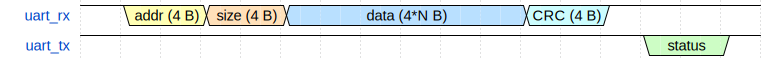
\includegraphics[width=\textwidth]{graphics/EduSoC_UART_Protocol.svg}
    \vspace{-1em}
    \caption{UART Bridge Protocol}
    \label{fig:uart_protocol}
\end{figure}
First, the starting memory address is sent (i.\,e. the address of the first word to be written). As described in Section \ref{sec:membus}, only 4-byte-aligned addresses are supported. This is followed by 4 bytes containing the size $N$ of the data to be written, \textbf{in units of 32 bit (4 byte) words} (\textit{not} bytes).

The next $N$ 32 bit words, i.\,e. $4 \cdot N$ bytes, are the actual data to be written, starting at the given address, with further words being written to the consecutively next memory addresses. Finally, the last 32 bit word is a CRC sum of the preceding data words (not including the address and size). The CRC algorithm used is CRC-32C (polynomial \ttt{0x1EDC6F41}, input and output reversed, initial value = final XOR = \ttt{0xFFFFFFFF}).

Once the bridge has received all of this data, it responds with a single byte indicating the status, which may be one of the following:\\
\begin{table}[H]
    \centering
    \begin{tabular}{|c|c|}\hline
        Value & Meaning \\\hline\hline
        0x59 & Success \\
        0x23 & CRC Mismatch \\
        0xE0 & Error \\
        Other & Unknown (error) \\\hline
    \end{tabular}
    \caption{UART Status Codes}
    \label{tab:uart_status}
\end{table}
Once a success or CRC mismatch status has been sent by the bridge, it is ready for a new transmission.
In the last two cases (error), the state of the UART bridge and the destination memory area is undefined, and the bridge may not respond to further UART transmissions. An external system reset is required to return to a known valid state.

In case of a CRC mismatch, data corruption during the transmission is possible. Note that this possibly corrupted data has been written to the destination memory area at this point, so it is recommended to retry the transmission to overwrite the corrupted data.

The EduSoC repository includes a Python script (\ttt{uart-programming/uart\_upload.py}) implementing this UART interface for the Digilent Arty S7 board. See the header comment in the script itself for more information.

\section{VGA Controller}\label{sec:vga}
EduSoC features a VGA video interface, requiring only an external DAC module for the analog color signals, for example the Digilent PmodVGA.
By default, it is configured for a 640x480 video output at 60 Hz refresh rate, where only the central 640x360 area is backed by actual pixel data.

The VGA controller is connected to the framebuffer memory, reading one byte (8 bits) of framebuffer data for each pixel, in typical scanline order, and generating all VGA interface signals from this data and its given pixel clock.
The pixel data format is RGB-332, so for each byte (= pixel), the upper three bits are the red intensity, the next three bits are the green intensity, and the lowest two bits are the blue intensity.

The framebuffer can be read and written to using the memory bus, like any other memory section, and changes to it will be visible on a connected screen immediately as soon as the changed pixels are drawn in the next frame. Note that, like any other EduSoC memory, the framebuffer contents are not affected by a system reset.